\documentclass{article} % use option titlepage to get the title on a page of its own.
\usepackage{polski}
\usepackage[utf8]{inputenc}
\usepackage{graphicx}
\usepackage[a4paper, total={7in, 10in}]{geometry}
\usepackage{listings}
\graphicspath{ {./images/} }
\title{Wskaźnik Giełdowy MACD}
\date{23.03.2018}
\author{Mateusz Buchajewicz}
\begin{document}
\maketitle
\section{Wprowadzenie}
Celem projektu było zaimplementowanie wskaźnika giełdowego MACD, wykorzystując dowolny język programowania.
Wskaźnik był sprawdzany na kursach 10 różnych walut w okresie od 01.04.2015 do 19.03.2019. 
Dane zaczerpnięto z serwisu money.pl. Na wykresach przedstawiono dane z kursu jena japońskiego. \\

\begin{figure}[h]
    \centering
    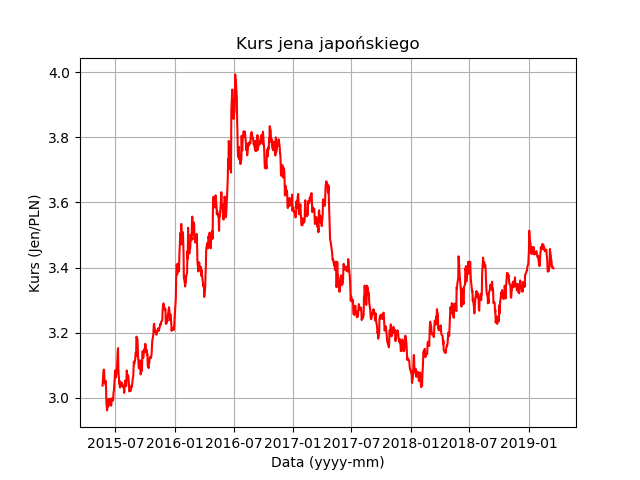
\includegraphics[scale=0.7]{wykres_kursu}
    \caption{Wykres kursu jena japońskiego w okresie od 01.04.2015 do 19.03.2018.}
\end{figure} 

Ze względu na niemożliwość obliczenia składowych wskaźnika MACD dla okresu 01.04.2015 - 10.05.2015
(ze względu na brak danych z dni poprzedzających ten okres), na późniejszych wykresach jest on pomijany. \\

Do implementacji wskaźnika wykorzystano język Python. Wykresy zostały narysowane z wykorzystaniem pakietu matplotlib.




\newpage

\section{Wskaźnik MACD}
\subsection{Podstawa teoretyczna}
Wskaźnik MACD składa się z dwóch wykresów: MACD oraz linii sygnałowej SIGNAL. 
Oba opierają się na wykładniczej średniej kroczącej, określonej wzorem: \\
\begin{equation}
    EMA_{N} = \frac{p_{0} + (1-\alpha)p_{1} + \dots + (1-\alpha)^N p_{N}}{(1-\alpha) + \dots + (1-\alpha)^N}
\end{equation}
gdzie: \\ \newline
$ \alpha = \frac{2}{N - 1} $ \\
$ N $ - liczba okresów \\
$ p_{i} $ - wartość danej sprzed $ i $ dni \\


Składowa MACD jest różnicą $ EMA_{12} - EMA_{26} $ obliczoną w oparciu o dane (w tym wypadku kurs jena japońskiego). 
Linia sygnałowa SINGAL jest obliczana jako $ EMA_{9} $ ze składowej MACD.

\subsection{Wykres składowych wskaźnika MACD}

\begin{figure}[h]
    \centering
    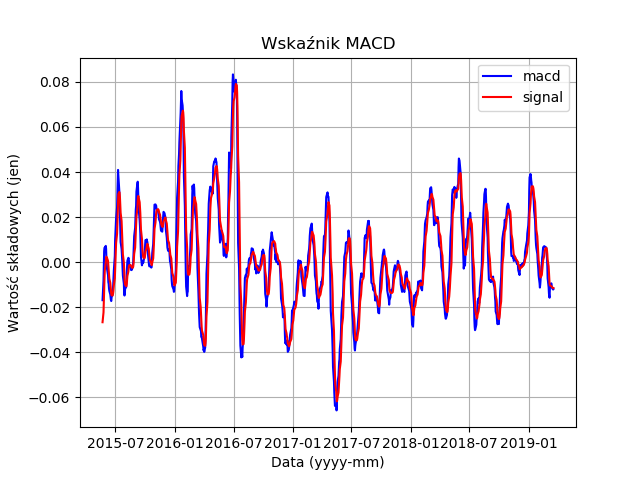
\includegraphics[scale=0.7]{images/wykres_macd.png}
    \caption{Wykres składowych wskaźnika MACD dla kursu jena japońskiego. Dane z okresu od 11.05.2015 do 19.03.2019}
\end{figure}

\newpage

\section{Analiza}

\begin{figure}[h]
    \centering
    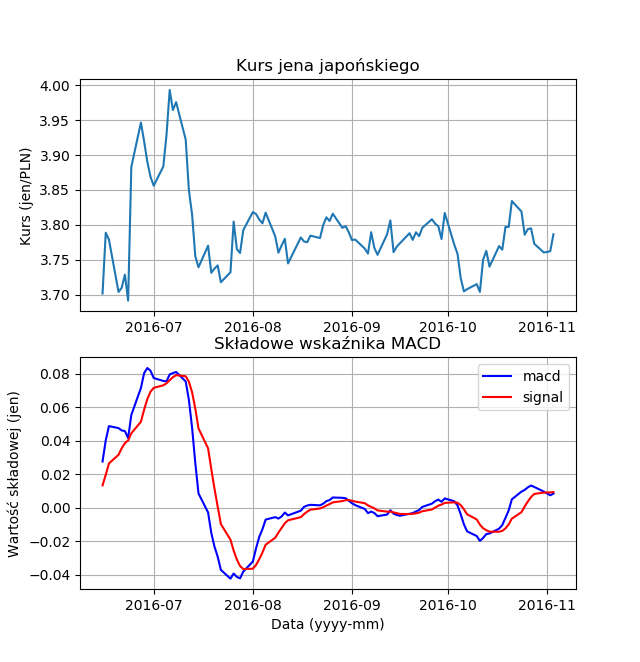
\includegraphics[scale=0.7]{images/wykres_bez_ulepszenia.png}
    \caption{Wykres kursu jena japońskiego i wskaźnika MACD w okresie 02.06.2016 - 20.10.2016}
\end{figure}


Warto zwrócić uwagę, iż w domyślnej wersji algorytmu sygnały zakupu i sprzedaży generowane są za każdym przecięciem 
linii sygnałowej SIGNAL i składowej MACD.
Taka konfiguracja pozwala na osiągnięcie około 6\% zysku. \\
Ograniczenie częstości wysyłania sygnałów pozwala na znaczące zwiększenie przychodów. Można to zrobić na przykład wysyłając sygnał
tylko wtedy, gdy wartość składowej MACD jest większa od 0 (dla sygnału zakupu), 
bądź mniejsza (dla sygnału sprzedaży). Potencjalne zwiększenie zysku obrazuje poniższa tabela: (Wszystkie dane są z okresu od 01.04.2015 do 19.03.2019. Źródło: money.pl) \\
\begin{center} 
    \begin{tabular}  { | c || c | c || c |  }
        \hline
        WALUTA & PRZED & PO & RÓŻNICA (punkty procenotowe) \\
        \hline
        \hline
        dolar amerykański & 5\% & 5\% & 0 \\
        \hline
        dolar hongkongski & 1\% & 5\% & +4 \\
        \hline
        euro & 3\% & 2\% & -1 \\
        \hline
        frank szwajcarski & -9\% & -4\% & +5 \\
        \hline
        jen japoński & 6\% & 20\% & +14 \\
        \hline
        korona norweska & 5\% & -9\% & -14 \\
        \hline
        peso & 3\% & -1\% & -4 \\
        \hline 
        real brazylisjki & -17\% & 16\% & +33 \\
        \hline
        ringgit malezyjski & -2\% & 6\% & +8 \\
        \hline 
        rubel rosyjski & 5\% & -18\% & -23 \\
        \hline
        \hline
        SUMA & 0\% & 22\% & +22 \\
        \hline
        ŚREDNIA & 0\% & 2.2\% & +2.2 \\
        \hline
    \end{tabular}
\end{center}
\newpage
\section{Wnioski}
Jak widać na powyższej tabeli, zbyt częste wykonywanie operacji sprzedaży / zakupu może zmniejszyć zyski,
 a nawet spowodować straty, co najlepiej obrazuje przykład reala brazylijskiego. Wprowadzenie dodatkowego ogranicznika wysyłania sygnałów zakupu średnio pozwala za zwiększenie zysku o około 20 punktów procentowych. W związku z tym należy stwierdzić,
  iż metoda wskaźnika giełdowego MACD lepiej nadaje się do inwestycji długoterminowych niż krótkoterminowych, 
  jest więc dość przydatna podczas analizy technicznej.

\end{document}